\section{Exact geometry: the order-four gems and the Siamese gems}
\label{sec:results}

All hull computations in this section are exact (integer or rational arithmetic); the methods are in \Cref{sec:appendix}, the scripts and data in the ancillary directory \texttt{anc/}.

\subsection{Geometry of the 880 order-4 gems}
\label{sec:gem-geometry-880}

There are $8$ magic squares of order $3$, all images of the Lo Shu under $D_4$, and $7{,}040$ of order $4$, forming $880$ $D_4$-orbits; the order-four squares are attributed to Fr\'enicle de Bessy (his list was published in 1693) and have been recounted by computer \cite{beck2010enumeration}.
Dudeney sorted them into twelve groups according to the pattern of complementary pairs $(a,17-a)$ \cite{dudeney1917amusements}; we use his groups only as a classical reference partition.
The number $275{,}305{,}224$ of essentially different order-five squares is due to Schroeppel (1973) \cite{gardner1976}; for $n\ge6$ exact counts are, to the author's knowledge, not available (see Trump's compilation \cite{trump2012enumeration}).

For each of the $880$ essentially different order-$4$ magic squares we computed the Magic Gem $\mathcal G(S)$ exactly
(integer facet planes, merged coplanar triangles, rational volumes; \Cref{sec:appendix}); Euler's relation holds for all
$880$ gems.  \Cref{fig:gem-geometry-880} and \Cref{tab:gem-fvectors} summarise the results.

\begin{table}[htbp]
\centering
\caption{Face structure of the $880$ order-$4$ gems by number of hull vertices $V$: number of squares, of distinct
combinatorial types (face lattices up to isomorphism), of distinct exact volumes, and of distinct $f$-vectors $(V,E,F)$.
The full list of the $39$ $f$-vectors with multiplicities is in the ancillary file \texttt{anc/results\_geometry.json}.}
\label{tab:gem-fvectors}
\small
\begin{tabular}{r rrrrrrrrr r}
\toprule
$V$ & 8 & 9 & 10 & 11 & 12 & 13 & 14 & 15 & 16 & all\\
\midrule
squares & 7 & 10 & 103 & 80 & 380 & 106 & 162 & 14 & 18 & 880\\
types   & 4 & 1 & 27 & 32 & 129 & 52 & 85 & 7 & 15 & 352\\
volumes & 4 & 5 & 51 & 33 & 111 & 40 & 65 & 6 & 14 & 155\\
$f$-vectors & 4 & 1 & 6 & 5 & 7 & 5 & 5 & 3 & 3 & 39\\
\bottomrule
\end{tabular}
\end{table}

\paragraph{Vertex counts, $f$-vectors, volumes.}
Between $8$ and all $16$ of the points are hull vertices; $V=12$ is modal ($380/880$).  There are $39$ distinct $f$-vectors,
from $(8,14,8)$ (one gem, square \#54) and $(8,16,10)$ (one gem) to $(16,36,22)$ (nine gems), the modal one being
$(12,26,16)$ ($164$ gems); the multiset of facet sizes (number of triangles, quadrilaterals, \dots) is determined by the
$f$-vector in every case.  The exact volume takes $155$ distinct values, from
$58$ (square \#427) to $292/3$ (square \#379), mean $84.05$.  The denominators are $1,2,3,6$: all three
coordinates of every point are half-odd integers when $n$ is even, so the translate of a gem by $(\frac12,\frac12,\frac12)$ is a
lattice polytope of $\Z^3$ and its volume lies in $\frac16\Z$.
Surface areas range from $116.5$ to $148.6$.

\paragraph{Combinatorial types.}
Two gems have the same combinatorial type if their vertex--facet incidence
structures (equivalently, their face lattices) are isomorphic.  Grouping by a
Weisfeiler--Lehman hash of the bipartite vertex--facet graph and confirming
every group by an explicit graph isomorphism test gives
\[
352\ \text{combinatorial types}
\]
among the $880$ gems (the hash was already exact: no hash class had to be
split).  Their sizes are very uneven; the number of types with $1,2,3,\dots$ members is
\[
\begin{array}{r|rrrrrrrrrrrrrr}
\text{squares per type} & 1&2&3&4&5&6&7&8&10&13&14&16&26&32\\\hline
\text{types} & 93&201&8&20&4&7&4&5&5&1&1&1&1&1
\end{array}
\]
(\Cref{fig:gem-geometry-880}c); the largest type, with $f=(10,22,14)$ (12 triangles,
2 quadrilaterals), is shared by $32$ squares, and the second largest,
$f=(12,24,14)$, by $26$.  The $7$ gems with $8$ vertices fall into $4$ types,
including a single $(8,14,8)$ gem with four triangular and four quadrilateral
faces (square \#54, Fig.~\ref{fig:gem-geometry-880}d) and four
$(8,18,12)$ gems sharing one simplicial type with $12$ triangular faces.  The $18$ gems with all $16$ points
extreme belong to $15$ types.

\paragraph{Congruence classes and injectivity.}
Two gems are \emph{congruent} if an isometry of $\mathbb R^3$ (rotations, reflections, translations) maps one onto the
other; since a distance-preserving bijection between finite point sets extends to an isometry, congruence is decided exactly
by testing for a bijection of hull-vertex sets preserving all integer squared distances (\Cref{sec:appendix}).

\begin{proposition}[class $\to$ gem]
\label{prop:gem-injective}
\begin{enumerate}
\item The $880$ hull-vertex sets are pairwise distinct: the map from
  $D_4$-classes of order-$4$ magic squares to hull-vertex sets (as subsets of
  $\mathbb R^3$) is injective.  (For the full $16$-point sets this is trivial, since the point set determines the
  arrangement.)
\item Up to congruence there are exactly $616$ gems.  The congruence classes
  are precisely the orbits of the complement map $S\mapsto 17-S$, which acts
  on gems as the reflection $z\mapsto -z$: $352$ squares are
  self-complementary (their gems have a non-trivial isometry,
  \Cref{thm:symmetry}) and the other $528$ form $264$ mirror pairs.  No two gems of
  non-complementary squares are congruent, not even as full $16$-point sets.
\end{enumerate}
\end{proposition}

Part (2) is the only failure of injectivity, and it is the expected one: $17-S$ is magic whenever $S$ is, and its gem is the
mirror image of $\mathcal G(S)$ in the plane $z=0$.  The $352$ self-complementary classes are exactly Dudeney's group III (the
$48$ associative squares) together with all $304$ squares of group VI \cite{dudeney1917amusements}.  The coincidence
$352=\#\{\text{types}\}=\#\{\text{self-complementary squares}\}$ is numerical only: the two partitions of the $880$ are different.

\paragraph{Dudeney groups.}
Crossing the hull-vertex count with Dudeney's twelve groups (table in the ancillary files) shows that geometry is only
loosely tied to Dudeney type: every group with more than eight members spans at least three vertex counts and at least $20$
combinatorial types; the $8$-vertex gems occur only in groups VI (three) and VIII (four).


The groups III and VI, the self-complementary ones, have only even vertex counts; this is \Cref{prop:facet-orbits}(3).

\begin{figure}[htbp]
\centering
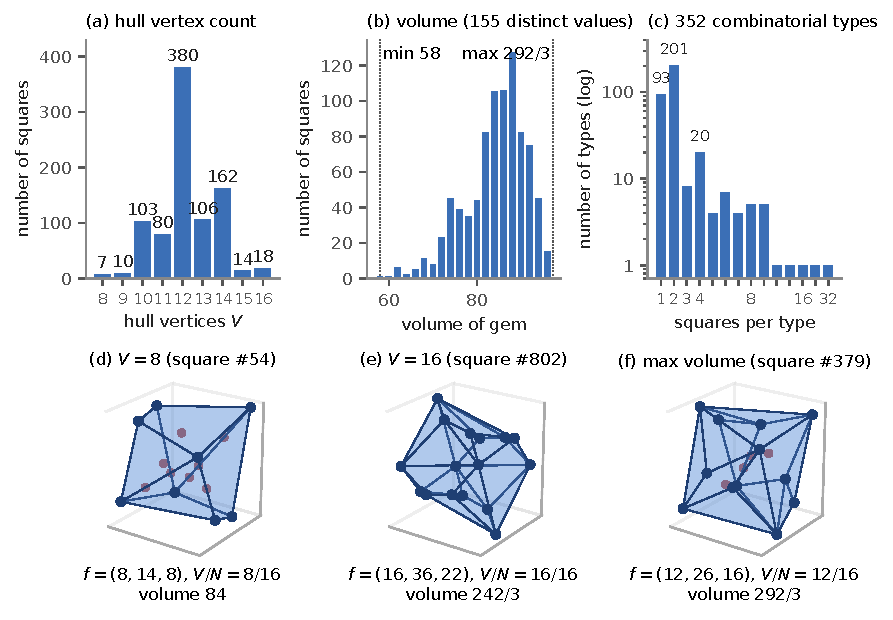
\includegraphics[width=0.9\textwidth]{figures/fig_gem_geometry_880.pdf}
\caption{Geometry of the $880$ order-$4$ Magic Gems.
(a)~Number of hull vertices ($8$ to $16$; modal value $12$).
(b)~Exact hull volume ($155$ distinct values between $58$ and $292/3$).
(c)~Sizes of the $352$ combinatorial types (logarithmic scale): $93$ types occur once, $201$
twice, and one type is shared by $32$ squares.
(d)--(f)~Three extreme gems, drawn with translucent faces after merging
coplanar triangles: the unique $(8,14,8)$ gem (square \#54; its four strictly interior points are red discs and its four boundary non-vertex points orange squares), a gem with all $16$ points extreme
(square \#802, D\"urer's square with its first two rows exchanged and its last two rows exchanged), and the gem of largest
volume (square \#379).}
\label{fig:gem-geometry-880}
\end{figure}

\paragraph{Named squares.}
The gems of the Lo Shu, of D\"urer's square and of the Siamese square of order $5$ have hull fractions $8/9$, $12/16$ and
$12/25$ and exact volumes $18$, $92$ and $830/3$.  D\"urer's own gem is centrally symmetric with twelve vertices, but exchanging its first two rows and
its last two rows (which preserves the magic property) gives a square whose gem has all sixteen points extreme (square \#802,
\Cref{fig:gem-geometry-880}e): the hull-vertex count is a property of the square, not of the Dudeney group or of the
construction method.

% ===========================================================================
\subsection{Extreme points and the bounding box}
\label{sec:box}

Let $B_n=[-\frac{n-1}2,\frac{n-1}2]^2\times[-\frac{N-1}2,\frac{N-1}2]$, a box of volume $(n-1)^2(N-1)$ that depends only on $n$.
The \emph{side lines} of the grid are its first and last rows and columns.

\begin{proposition}[Bounding box and forced vertices]
\label{prop:box}
Let $S$ be any arrangement of order $n\ge2$.
\begin{enumerate}\setlength\itemsep{0pt}\setlength\topsep{2pt}
\item $\mathcal G(S)\subseteq B_n$.
\item The points carrying the entries $1$ and $N$ are the only points on the planes $z=\mp\frac{N-1}2$, and they are vertices of $\mathcal G(S)$.
\item The points over the four corner cells of the grid are vertices.
\item For each of the four side lines, the points over its cells carrying the smallest and the largest entry of that line are vertices.
\end{enumerate}
\end{proposition}

\begin{proof}
(1) $|x_{ij}|,|y_{ij}|\le\frac{n-1}2$ and $1\le s_{ij}\le N$, and $B_n$ is convex.
A point that is the unique maximiser over $\{\mathbf p_{ij}\}$ of a linear functional is a vertex.
(2) The entries are distinct, so $z$ is uniquely minimal where $s=1$ and uniquely maximal where $s=N$.
(3) On the grid the functional $-x+y$ attains its maximum $n-1$ only at the top-left cell, and similarly for the other corners.
(4) Take the left column, where $x=-\frac{n-1}2$ and the other columns have $x\ge-\frac{n-1}2+1$.
For $\varepsilon=1/N$ the functional $-x+\varepsilon z$ has, on points of the column, values greater than $\frac{n-1}2-\frac12$ and, on all other points, values at most $\frac{n-1}2-1+\frac12$; so its maximiser lies in the column and is the point of largest height there, which is unique.
Replacing $\varepsilon z$ by $-\varepsilon z$ gives the point of smallest height, and the other three sides are obtained by applying elements of $D_4$.
\end{proof}

The vertices named in (2)--(4) number at least $4$ and at most $14$; for $n=4$ they number between $4$ and $13$ over the $880$ gems, and nothing more is forced (exact computation, \texttt{anc/box\_and\_classes.py}): the only cells carrying a vertex in all $880$ gems are the four corners, and the only entries that always label a vertex are $1$ and $16$.
In particular $2$ and $N-1$ are not forced: in eight gems the point carrying $2$ is a boundary non-vertex point, for instance for square \#593, $\begin{smallmatrix}4&1&16&13\\5&15&2&12\\14&8&9&3\\11&10&7&6\end{smallmatrix}$, and the complement $17-S$ (the mirror image, \Cref{lem:complement}) has the same property for $15$.
The twelve vertices of a Siamese gem (\Cref{prop:siamese-12}) are its forced vertices.

\Cref{tab:box} gives the volume of the order-four gems as a fraction of $\operatorname{vol}B_4=135$ and the numbers $I$ and $B$ of strictly interior and boundary non-vertex points (exact computation).
Gems fill between $58/135\approx43\%$ and $292/405\approx72\%$ of the box, on average $2219/3564\approx62\%$.
At most four points are strictly interior, while one gem has $I=0$, $B=6$.

\begin{table}[htbp]
\centering
\caption{Order-four gems: volume as a fraction of the box $B_4$ (exact; rounded), by number $V$ of vertices, and numbers of gems with $k$ strictly interior points ($I=k$) and with $k$ boundary non-vertex points ($B=k$).}
\label{tab:box}
\small
\begin{tabular}{r rrrrrrrrr r}
\toprule
$V$ & 8 & 9 & 10 & 11 & 12 & 13 & 14 & 15 & 16 & all\\
\midrule
min & .622 & .588 & .481 & .549 & .430 & .456 & .452 & .498 & .449 & .430\\
mean & .642 & .623 & .631 & .630 & .634 & .614 & .608 & .560 & .536 & .623\\
max & .648 & .667 & .701 & .699 & .721 & .688 & .691 & .615 & .598 & .721\\
\bottomrule
\end{tabular}

\medskip
\begin{tabular}{r rrrrrr}
\toprule
$k$ & 0 & 1 & 2 & 3 & 4 & 6\\
\midrule
gems with $I=k$ & 37 & 32 & 353 & 178 & 280 & 0\\
gems with $B=k$ & 357 & 204 & 257 & 40 & 21 & 1\\
\bottomrule
\end{tabular}
\end{table}

% ===========================================================================
\subsection{Lattice structure and Ehrhart polynomials}
\label{sec:ehrhart}

For even $n$ all coordinates of every $\mathbf p_{ij}$ are half-odd integers, so $Q(S)=\mathcal G(S)+(\frac12,\frac12,\frac12)$ is a lattice polytope; any other lattice translate has the same Ehrhart polynomial $L_S(t)=\#(tQ\cap\Z^3)=\operatorname{vol}(\mathcal G)\,t^3+c_2t^2+c_1t+1$ \cite{beck2007computing}, and $L_S$ is the same for all images $gS$, $g\in D_4$, since $\hat g$ preserves $\Z^3$ up to an integer translation of $Q$.
Writing $\sum_{k\ge0}L_S(k)t^k=(h^*_0+h^*_1t+h^*_2t^2+h^*_3t^3)/(1-t)^4$, the $h^*_i$ are non-negative integers \cite{stanley1980decompositions}, $h^*_0=1$, $\sum h^*_i=6\operatorname{vol}$, and $h^*_3$ is the number of interior lattice points of $Q$ \cite{beck2007computing}.

\emph{Exact computation} (\texttt{anc/ehrhart\_880.py}; lattice points of $tQ$ counted for $t\le6$, the cubic interpolated from $t\le3$ and checked at $t=4,5,6$, with $h^*_3$ checked against the interior count and $\sum h^*_i$ against $6\operatorname{vol}$).
Over the $880$ gems, $h^*_1\in[70,136]$, $h^*_2\in[233,403]$ and $h^*_3\in[34,52]$.
There are $554$ distinct Ehrhart polynomials, against $616$ congruence classes, $352$ combinatorial types, $39$ $f$-vectors and $155$ volumes: congruent gems (complement partners; the reflection $z\mapsto-z$ followed by an integer translation is a unimodular affine map of $\Z^3$) have equal polynomials, but non-congruent gems can share one, and $L_S$ is determined neither by the $f$-vector (it takes several values on $29$ of the $39$ $f$-vectors), nor by the combinatorial type ($81$ of $352$ types), nor by the volume ($104$ of $155$ volumes).
For the Lo Shu square (odd order: the gem itself is a lattice polytope) $L(t)=1+t+13t^2+18t^3$ and $h^*=(1,29,73,5)$; for D\"urer's square $L(t)=1-3t+44t^2+92t^3$ and $h^*=(1,130,377,44)$; the leading coefficients are the volumes $18$ and $92$.

% ===========================================================================
\subsection{Siamese gems have twelve vertices}
\label{sec:siamese-gems}

For the Siamese (de la Loub\`ere) squares of odd order the hull-vertex count
does not grow with $n$.  We computed the gems for $n=3,5,\dots,21$: the Lo Shu
gem has $f=(8,16,10)$, and every Siamese gem with $n\ge5$ has
$f=(12,26,16)$ with $12$ triangular and $4$ quadrilateral facets, so the hull
fraction $12/n^2$ tends to zero.  This is a
theorem, with a short computer-assisted proof.

\begin{proposition}[Siamese gems]
\label{prop:siamese-12}
Let $n=2m+1\ge5$ and let $S$ be the Siamese square of order $n$ ($1$ in the
middle cell of the top row, successive entries one step up and to the right
modulo $n$, one step down when blocked).  Then $\mathcal G(S)$ has exactly $12$
vertices, $26$ edges and $16$ facets ($12$ triangles, $4$ quadrilaterals).
With $0$-indexed cells $(i,j)$ and $c=(n^2+1)/2$, the vertices are the
points over the cells
\[
\begin{array}{lll}
(0,0)\colon c+m+2, & (0,m-1)\colon n^2-1, & (0,m)\colon 1, \\
(0,2m)\colon c+m, & (m-1,0)\colon n^2-m, & (m,0)\colon m+2, \\
(m,2m)\colon n^2-m-1, & (m+1,2m)\colon m+1, & (2m,0)\colon c-m, \\
(2m,m)\colon n^2, & (2m,m+1)\colon 2, & (2m,2m)\colon c-m-2,
\end{array}
\]
i.e.\ the four corners, and on each side of the square the two cells holding
the side's extreme values.  For $n=3$ the same construction gives the Lo Shu
gem, with $8$ vertices (all cells except the centre).
\end{proposition}

\begin{proof}
\emph{Step 1: closed form.}  Write $\langle t\rangle\in\{0,\dots,n-1\}$ for
$t\bmod n$.  We claim $s(i,j)=n\langle i+j-m\rangle+\langle i+2j-2m\rangle+1$.
Indeed, along a run of $n$ consecutive entries the move $(i,j)\to(i-1,j+1)$
fixes $i+j$ and increases $i+2j$ by $1$ modulo $n$, while the ``blocked''
move $(i,j)\to(i+1,j)$ increases both $i+j$ and $i+2j$ by $1$; the entry $1$
sits at $(0,m)$ where both expressions vanish.  Hence by induction the entry
$k$ lies in a cell with $\langle i+j-m\rangle=\lfloor (k-1)/n\rfloor$ and
$\langle i+2j-2m\rangle=\langle k-1\rangle$; since
$(i,j)\mapsto(i+j,\,i+2j)$ is a bijection of $\mathbb Z_n^2$ (determinant
$1$), this determines the cell, which proves the claim.

\emph{Steps 2 and 3 (sketch; details in \Cref{sec:app_siamese}).}  With $m=(n-1)/2$, $x=j-m$, $y=m-i$, the closed form gives
$z=L(x,y)+n\,\zeta(x,y)$ with $L$ affine and
$\zeta=-n\lfloor(x-y+m)/n\rfloor-\lfloor(2x-y+m)/n\rfloor\in\{\pm(n+1),\pm1,0\}$.
The affine bijection $\Phi(x,y,z)=(x,y,(z-L)/n)$ preserves the face lattice and the vertex cells, and
$\Phi(\mathcal G(S))$ is the convex hull of the lattice points of five convex lattice polygons at the five heights $\zeta$:
two triangles $T$, $B=-T$ at $\zeta=\pm(n+1)$, two triangles $U$, $D=-U$ at $\zeta=\pm1$, and a parallelogram $M$ at
$\zeta=0$ (\Cref{fig:siamese-layers}a).  Sixteen explicit planes, eight of them and their images under $(x,y,\zeta)\mapsto
-(x,y,\zeta)$, are shown to support the convex hull of twelve named points $v_1,\dots,v_{12}$---the three corners of $T$ and
of $B$, one corner each of $U$ and $D$, and the four corners of $M$---in facets that close up into a surface with
$(V,E,F)=(12,26,16)$ closed under edge-adjacency, hence all facets (so $P=Q$), and every vertex of every layer polygon satisfies all sixteen inequalities
(\Cref{fig:siamese-layers}b).  These are finitely many polynomial identities and inequalities in $m$, verified exactly for all
integers $m\ge2$ by the script \texttt{siamese\_proof.py}.  Hence $\Phi(\mathcal G(S))=\operatorname{conv}\{v_1,\dots,v_{12}\}$,
and mapping back by $\Phi^{-1}$ gives the statement; for $m=1$ the four triangles degenerate to points and the same argument
gives the $8$-vertex Lo Shu gem.
\end{proof}

\begin{figure}[htbp]
\centering
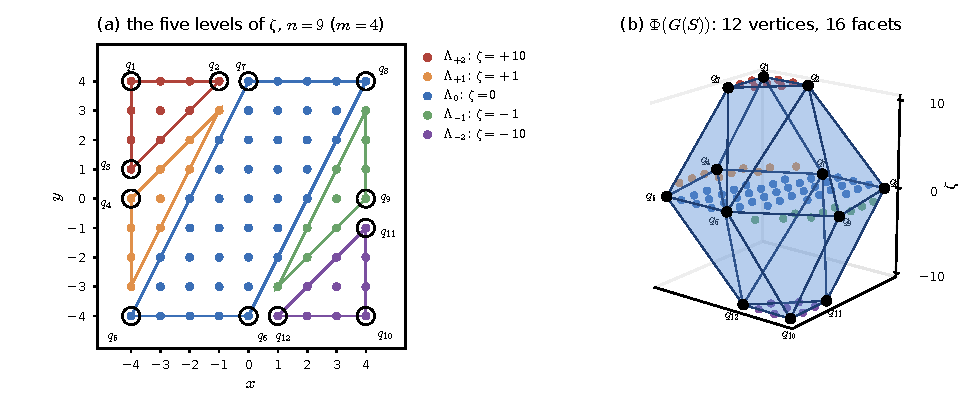
\includegraphics[width=0.88\textwidth]{figures/fig_siamese_layers.pdf}
\caption{The Siamese gem of order $n=9$ after the affine reduction of \Cref{prop:siamese-12}.
(a)~The $81$ cells in the $(x,y)$-plane coloured by the layer value $\zeta\in\{+10,+1,0,-1,-10\}$, with the five lattice
polygons $T,U,M,D,B$ outlined and the twelve vertex cells $v_1,\dots,v_{12}$ circled.
(b)~The reduced polytope $\Phi(\mathcal G(S))=\operatorname{conv}\{(x,y,\zeta)\}$ with its $12$ vertices and $16$ facets
($12$ triangles, $4$ quadrilaterals); the shapes of the layers do not depend on $n$ except through scale, which is why the
combinatorial type is constant for all odd $n\ge5$.}
\label{fig:siamese-layers}
\end{figure}
